The experience required to reach a level $L$ is given by,
\begin{align}\label{eq:xp_given_level}
	\mathcal{L}^{-1}(L) &\equiv \left \lfloor \frac{1}{4} \sum_{l=1}^{L-1} \left \lfloor l + 300\cdot2^{l/7} \right \rfloor \right\rfloor\\
	&\approx \frac{1}{8}\left( L^2 - L + 600\frac{2^{L/7} - 2^{1/7}}{2^{1/7}-1}\right).
\end{align}
The level of a skill with $E$ experience is defined as:
\begin{align}\label{eq:level_given_xp}
	\mathcal{L}(E).
\end{align}
No analytic form has been found for this equation, however it can be straightforwardly evaluated by numerically inverting Eq.~(\ref{eq:xp_given_level}) or by building lookup tables.

The level equation itself is exponentially slow, and this effect extends to the overall time to max all skills. For example, one youtuber, WildMudKip provides total level and date stamps through their \href{https://www.youtube.com/watch?v=MiTp-06zJHk&list=PL4Ct8chrkvPgti4HYTZFo7FSfxlLlptbN&ab_channel=WildMudkip}{HCIM youtube series}, by scraping this data, Fig.~\ref{fig:maxing_time} now shows that the total level over time is also logarithmic.


\begin{figure}
	\centering
	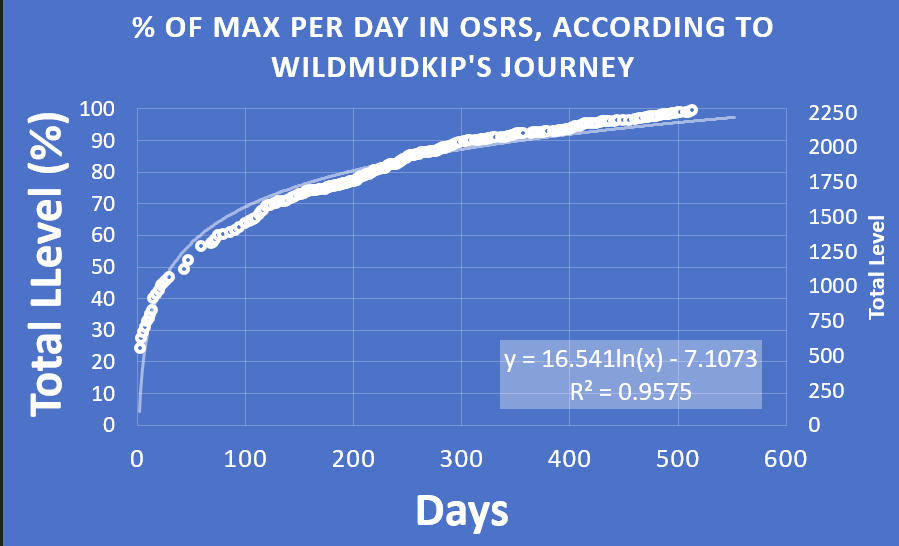
\includegraphics[width=\linewidth]{img/general/wildmudkip_maxing.png}
	\caption{
		Youtuber WildMudKip's hardcore ironman levels over time reveal an logarithmically slow progression. Near optimal play and consistent upload and play time are all reasonable assumptions.
	}
	\label{fig:maxing_time}
\end{figure}
